\documentclass{standalone}

\usepackage{tikz} % Allows creation of tikz pictures
\usetikzlibrary{arrows,shapes,snakes}

\begin{document}
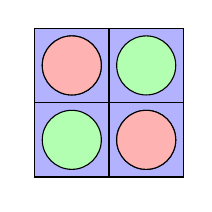
\begin{tikzpicture}[scale=0.75, every node/.style={scale=1}]
        \foreach \x in {0,1.26}
        \foreach \y in {0,1.26}
        \filldraw[xshift=\x cm, yshift=\y cm, fill=blue!30!white, 
        draw=black] (0, 0) rectangle (1.26,1.26) node[pos=.5] {};
        \foreach \x in {0,1.26}
        \foreach \y in {0,1.26}
        \filldraw[xshift=\x cm, yshift=\y cm, fill=green!30!white, 
        draw=black] (.63,.63) circle (.5) node[pos=.5] {};
        \filldraw[xshift=0 cm, yshift=1.26 cm, fill=red!30!white, 
        draw=black] (.63,.63) circle (.5) node[pos=.5] {};
        \filldraw[xshift=1.26 cm, yshift=0 cm, fill=red!30!white, 
        draw=black] (.63,.63) circle (.5) node[pos=.5] {};
    \end{tikzpicture}
\end{document}